\documentclass[xetex,mathserif,serif,handout]{beamer}

\usepackage{xunicode}
\usepackage{xltxtra}
\usepackage{color}
\usepackage{url}
\usepackage{listings}
\usepackage{fontspec}
\usepackage{geometry}
\usepackage{lastpage}
\usepackage{fancyhdr}
\usepackage{amsmath}
\usepackage{amsthm}
\usepackage{amssymb}
\usepackage{blkarray}
\usepackage{multicol}
\usepackage{relsize}

\definecolor{solarized@base03}{HTML}{002B36}
\definecolor{solarized@base02}{HTML}{073642}
\definecolor{solarized@base01}{HTML}{586e75}
\definecolor{solarized@base00}{HTML}{657b83}
\definecolor{solarized@base0}{HTML}{839496}
\definecolor{solarized@base1}{HTML}{93a1a1}
\definecolor{solarized@base2}{HTML}{EEE8D5}
\definecolor{solarized@base3}{HTML}{FDF6E3}
\definecolor{solarized@yellow}{HTML}{B58900}
\definecolor{solarized@orange}{HTML}{CB4B16}
\definecolor{solarized@red}{HTML}{DC322F}
\definecolor{solarized@magenta}{HTML}{D33682}
\definecolor{solarized@violet}{HTML}{6C71C4}
\definecolor{solarized@blue}{HTML}{268BD2}
\definecolor{solarized@cyan}{HTML}{2AA198}
\definecolor{solarized@green}{HTML}{859900}
\definecolor{yaleblue}{HTML}{0E4C92}

\newcommand{\yellow}[1]{\textcolor{solarized@yellow}{#1}}
\newcommand{\orange}[1]{\textcolor{solarized@orange}{#1}}
\newcommand{\red}[1]{\textcolor{solarized@red}{#1}}
\newcommand{\magenta}[1]{\textcolor{solarized@magenta}{#1}}
\newcommand{\violet}[1]{\textcolor{solarized@violet}{#1}}
\newcommand{\blue}[1]{\textcolor{solarized@blue}{#1}}
\newcommand{\cyan}[1]{\textcolor{solarized@cyan}{#1}}
\newcommand{\green}[1]{\textcolor{solarized@green}{#1}}
\newcommand{\yblue}[1]{\textcolor{yaleblue}{#1}}

\setbeamertemplate{navigation symbols}{}
% \setbeamerfont{title}{family=\old}
% \setbeamerfont{author}{family=\tfont}%
% \setbeamerfont{frametitle}{family=\oldA}
% \setbeamerfont{date}{family=\dfont}

\setbeamertemplate{itemize items}{--}
\setbeamercolor*{item}{fg=black}

\defaultfontfeatures{Mapping=tex-text}
\hypersetup{pdfstartview={FitH}}

\newcommand{\old}[1]{\fontspec[Alternate=1,Ligatures={Common}]{Hoefler Text}\fontsize{18pt}{30pt}\selectfont #1}%
\newcommand{\oldA}[1]{\fontspec[Alternate=1,Ligatures={Common, Rare}]{Hoefler Text}\fontsize{12pt}{15pt}\selectfont #1}%
\newcommand{\oldB}[1]{\fontspec[Ligatures={Common}]{Didot}\fontsize{12pt}{15pt}\color{solarized@base02}\selectfont #1}%
\newcommand{\tfont}[1]{\fontspec[Alternate=1,Ligatures={Common}]{Hoefler Text}\fontsize{12pt}{20pt}\selectfont #1}%
\newcommand{\dfont}[1]{\fontspec[Ligatures={Common}]{Didot}\fontsize{12pt}{12pt}\selectfont #1}%

\newcommand{\minimize}{\mathop{\mathrm{minimize}}}
\newcommand{\argmin}{\mathop{\mathrm{arg\,min}}}
\newcommand{\argmax}{\mathop{\mathrm{arg\,max}}}
\newcommand{\st}{\mathop{\mathrm{subject\,\,to}}}

\newcommand\independent{\protect\mathpalette{\protect\independenT}{\perp}}
\def\independenT#1#2{\mathrel{\rlap{$#1#2$}\mkern2mu{#1#2}}}

\setlength{\parindent}{0pt}
\setlength{\parskip}{12pt}

\setromanfont [Ligatures={Common}, Numbers={OldStyle}, Variant=01,
 BoldFont={LinLibertine_RB.otf},
 ItalicFont={LinLibertine_RI.otf},
 BoldItalicFont={LinLibertine_RBI.otf}
 ]{LinLibertine_R.otf}


\usepackage{hyperref}
\usepackage{listings}
\usepackage{dsfont}
\usepackage{tikz}
\usepackage{pgfplots}
\usetikzlibrary{patterns}
\usetikzlibrary{shapes}
\usetikzlibrary{calc}
\pgfplotsset{compat=1.11}

% commands
\newcommand{\bc}{\begin{center}}
\newcommand{\ec}{\end{center}}
\newcommand{\bb}[1]{\begin{block}{#1}}
\newcommand{\eb}{\end{block}}
\newcommand{\bi}{\begin {itemize}}
\newcommand{\ei}{\end{itemize}}
\newcommand{\be}{\begin {enumerate}}
\newcommand{\ee}{\end{enumerate}}
\DeclareMathOperator*{\plim}{plim}

% beamer settings
\usecolortheme[named=black]{structure}


\begin{document}
%===========================================================
\begin{frame}[fragile] \frametitle{}

\vfill

{\fontsize{0.7cm}{0cm}\selectfont Prediction, Estimation, and Attribution}\\
\vspace{0.5cm}

Statistical Learning\\
CLAMSES - University of Milano-Bicocca\\

\vspace{2cm}

\begin{minipage}{0.6\textwidth}
Aldo Solari
\end{minipage}

\end{frame}
%===========================================================
\begin{frame}[fragile]

\centering 
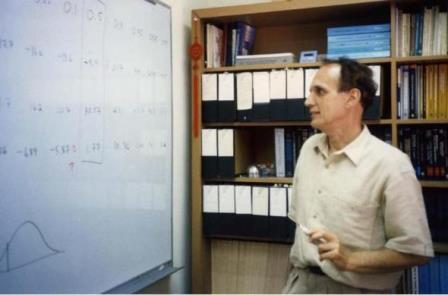
\includegraphics[scale=1]{images/1996_Efron-office}\\
{\tiny Bradley Efron working in his classic office, circa 1996.}

\end{frame}
%===========================================================
\begin{frame}[fragile]\frametitle{References}

\bi
\item \href{https://statprize.org/}{International Prize in Statistics 2019}
\item \href{https://www.fox.temple.edu/wp-content/uploads/2021/07/Efron-2020-JASA-wdiscussion.pdf}{Efron, B. (2020). Prediction, Estimation, and Attribution. Journal of the American Statistical Association, 115(530), 636-655.} With Discussion and Rejoinder.
\item \href{https://efron.ckirby.su.domains/talks/2019Predict-Estimat-Attribut.pdf}{Slides}
\item \href{https://drive.google.com/file/d/1uknyN7L8rIPCcyxGoXkMlVRE8lh5RFrm/view}{Recorded presentation} for the 62nd ISI World Statistics Congress in Kuala Lumpur [46 mins]
\ei

\end{frame}
%===========================================================
\begin{frame}[fragile]\frametitle{Outline}

\be
\item Introduction
\item Surface Plus Noise Models
\item The Pure Prediction Algorithms
\item A Microarray Prediction Problem
\item Advantages and Disadvantages of Prediction
\item The Training/Test Set Paradigm
\item Smoothness
\item A Comparison Checklist
\item TraditionalMethods in the Wide Data Era
\item Two Hopeful Trends
\ee

\end{frame}
%===========================================================
\begin{frame}[fragile]\frametitle{Regression\\
Gauss (1809), Galton (1877)}

What are the three important statistical tasks in regression?

\end{frame}
%===========================================================
\begin{frame}[fragile]
\begin{itemize}
\item \emph{Prediction: the prediction of new cases}

e.g. random forests, boosting, support vector machines,
neural nets, deep learning

\item \emph{Estimation: the
estimation of regression surfaces}

e.g. OLS, logistic regression, GLM: MLE

\item \emph{Attribution: the assignment of significance
to individual predictors}

e.g. ANOVA, lasso, Neyman Pearson
\end{itemize}

\end{frame}
%===========================================================
\begin{frame}[fragile]

How do the pure prediction algorithms relate to traditional
regression methods?

That is the central question pursued in
what follows.

\end{frame}
%===========================================================
\begin{frame}[fragile]

\bi
\item[2.] Surface Plus Noise Models
\ei

\end{frame}
%===========================================================
\begin{frame}[fragile]

We will assume that the data $\mathbf{d}$ available to the statistician
has this structure:
$$\mathbf{d} = \{(x_i,y_i), i=1,\ldots,n\}$$
\bi
\item  $x_i$ is a $p$-dimensional vector of predictors taking its value
in a known space $\mathcal{X}$ contained in $\mathbb{R}^p$;
\item $y_i$ is a real valued response;
\item the $n$ pairs are assumed to be independent of each
other.
\ei
More concisely we can write
$$\mathbf{d} = \{\mathbf{x},\mathbf{y}\}$$
where $\mathbf{x}$ is the $n\times p$ matrix having $x_i^t$ as the $i$th row, and $\mathbf{y}=(y_1,\ldots,y_n)^t$.


\end{frame}
%===========================================================
\begin{frame}[fragile]

\bi
\item The regression model is
\begin{eqnarray}
y_i = s(x_i,\beta) + \epsilon_i \quad i=1,\ldots,n
\end{eqnarray}
$\epsilon_i \stackrel{\mathrm{iid}}{\sim}\mathcal{N}(0,\sigma^2)$
where $s(x,\beta)$ is some functional form that, for any fixed
value of the parameter vector $\beta$, gives expectation $\mu=s(x,\beta)$ as a function of $x\in \mathcal{X}$; 

\item The \emph{regression surface} is
$$\mathcal{S}_\beta = \{\mu=s(x,\beta), x\in \mathcal{X}\}$$
Most traditional regression methods depend on some sort of
surface plus noise formulation;

\item The surface describes the scientific truths
we wish to learn, but we can only observe points on the surface
obscured by noise;

\item The statistician’s traditional estimation task is to learn as much as possible about the surface from the
data $\mathbf{d}$.
\ei

\end{frame}
%===========================================================
\begin{frame}[fragile]

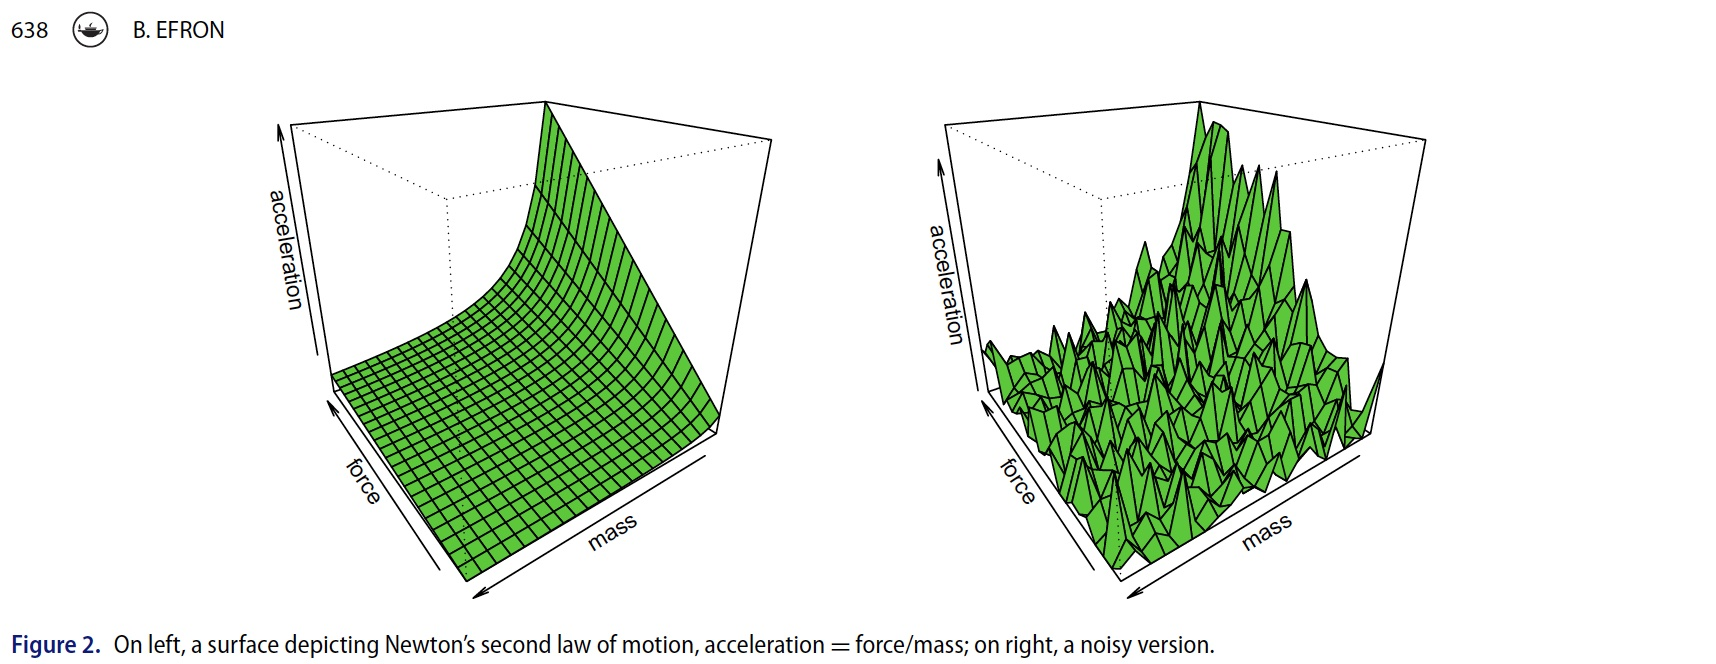
\includegraphics[scale=.2]{images/Figure_2}

\end{frame}
%===========================================================
\begin{frame}[fragile]\frametitle{Cholesterol data}

\bi
\item Cholestyramine, a proposed cholesterol lowering drug, was administered to 164 men for an average of seven years each.

\item The response variable is a man's decrease in cholesterol level over the course of the experiment.

\item The single predictor is compliance, the fraction of intended dose actually taken (standardized)

\item https://hastie.su.domains/CASI\_files/DATA/cholesterol.html
\ei

\end{frame}
%===========================================================
\begin{frame}[fragile]

\centering
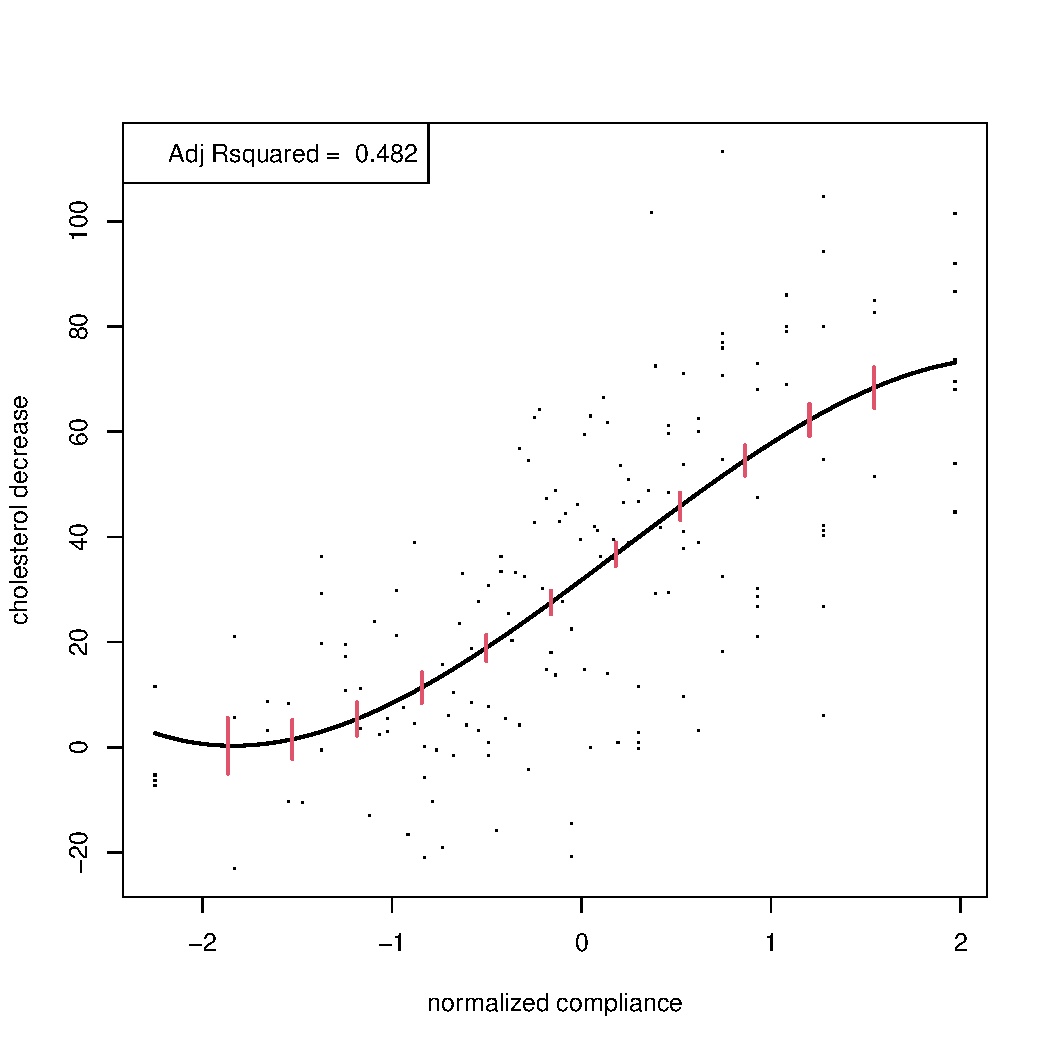
\includegraphics[scale=.5]{images/Figure_1}

\end{frame}
%===========================================================
\end{document}










